\documentclass[titlepage]{article}
\usepackage[utf8]{inputenc}
\usepackage{hyperref}
\usepackage{float}
\restylefloat{figure}
\usepackage{subcaption}
\usepackage{amsmath}
\usepackage{amssymb}
\usepackage{minted}
\usepackage{graphicx}
\DeclareGraphicsExtensions{.eps}
\usepackage{fancyhdr}
\pagestyle{fancy}
\lhead{Fractals and the Beauty of Nature}
\author{Chanthosh Sivanandam \\ Erik Andersen \\ Henrik Flindt }
\title{Fractals and the Beauty of Nature \\ DM550 - Fall Project 2017}
\begin{document}
\maketitle
\section{Sierpinsky Triangle}
\subsection{Specification and design}
We began by trying to implement an algorith for the Sierpinsky triangle which was build upon the idea of placing inverted triangles inside other triangles. It turned out to be overly complicated, but it yielded som rather interesting results, which can be seen here:
\begin{figure}[H]
  \centering
  \begin{subfigure}[b]{0.4\textwidth}
    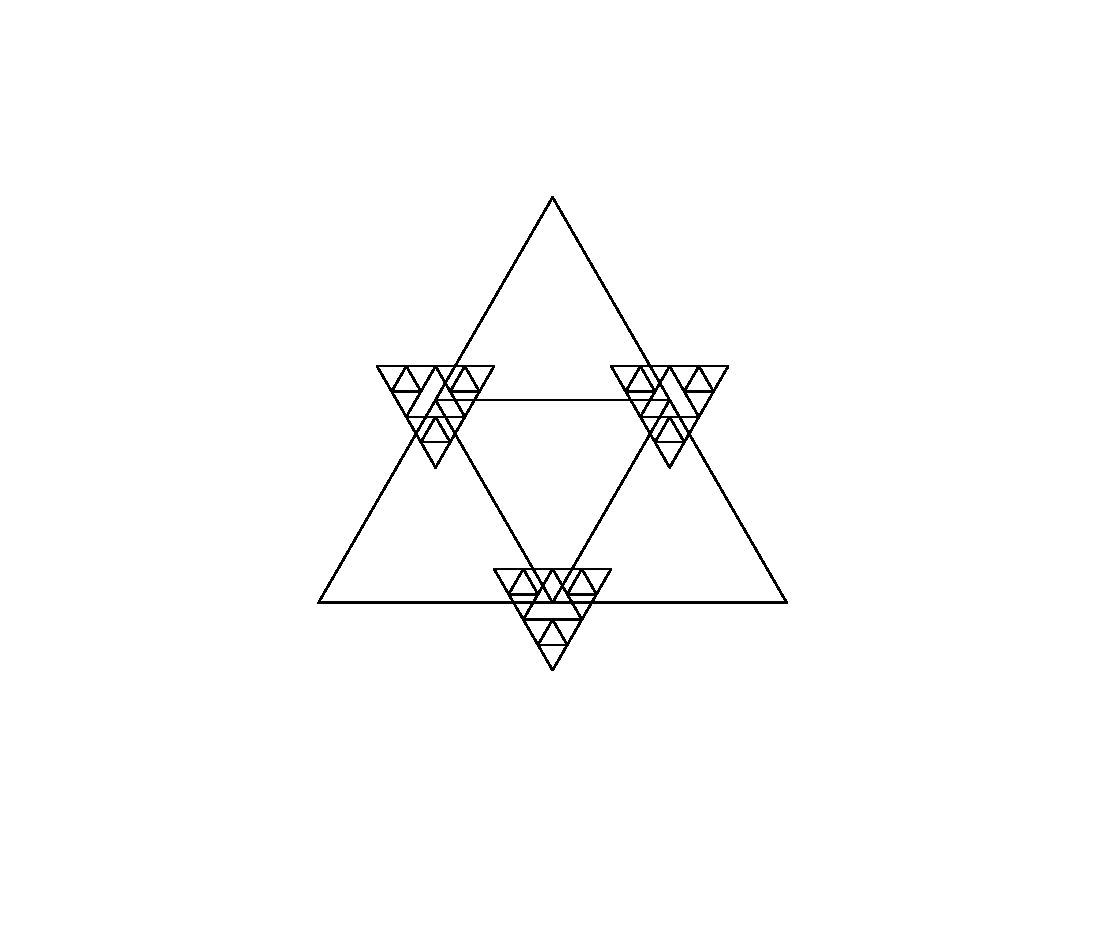
\includegraphics[width=\textwidth]{wrongtriangle}
    \caption{An unsuccesful attempt}
  \end{subfigure}
  \begin{subfigure}[b]{0.5\textwidth}
    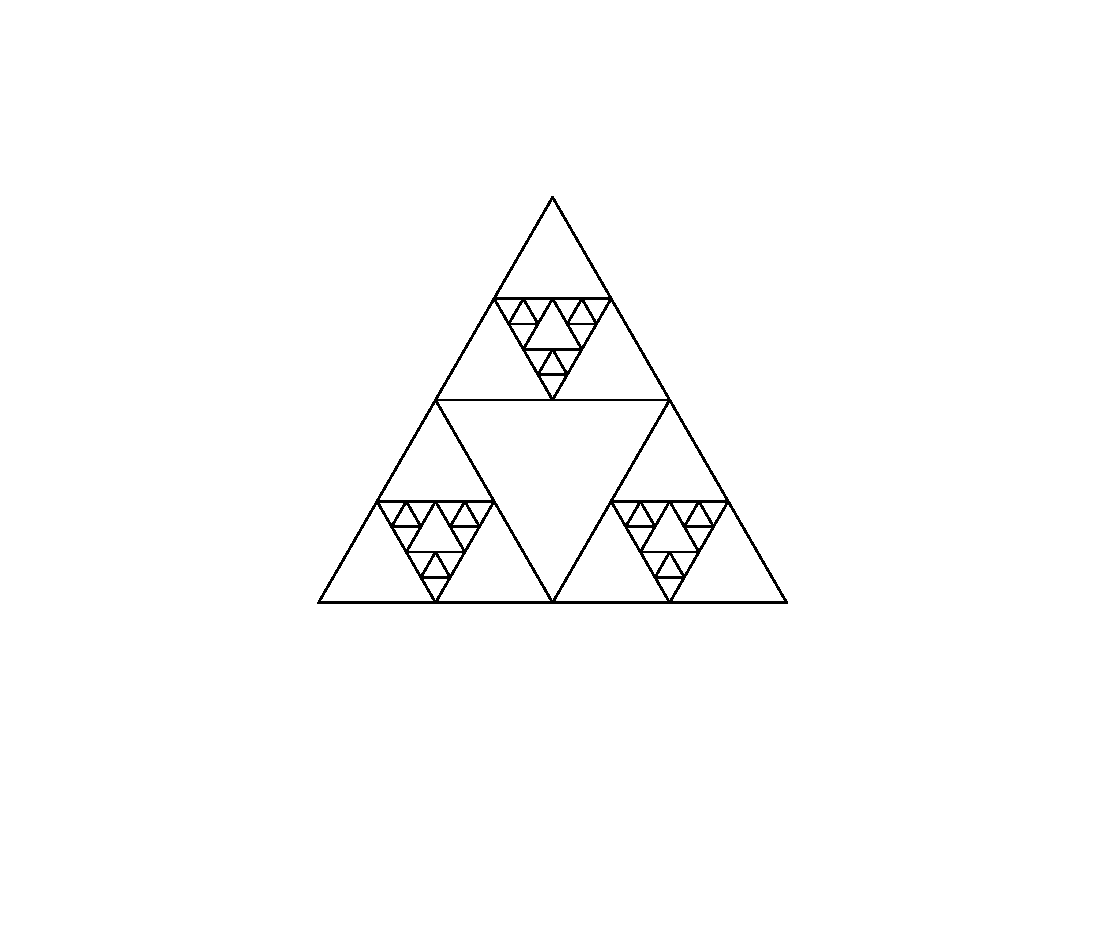
\includegraphics[width=\textwidth]{wrongtriangle2}
    \caption{Another unsuccesful attempt}
  \end{subfigure}
\end{figure}
After meddling around for some time, we decided to go with a more convenient approach, and quickly came up with a succesful algorithm, that gave the expected result.
\begin{figure}[H]
  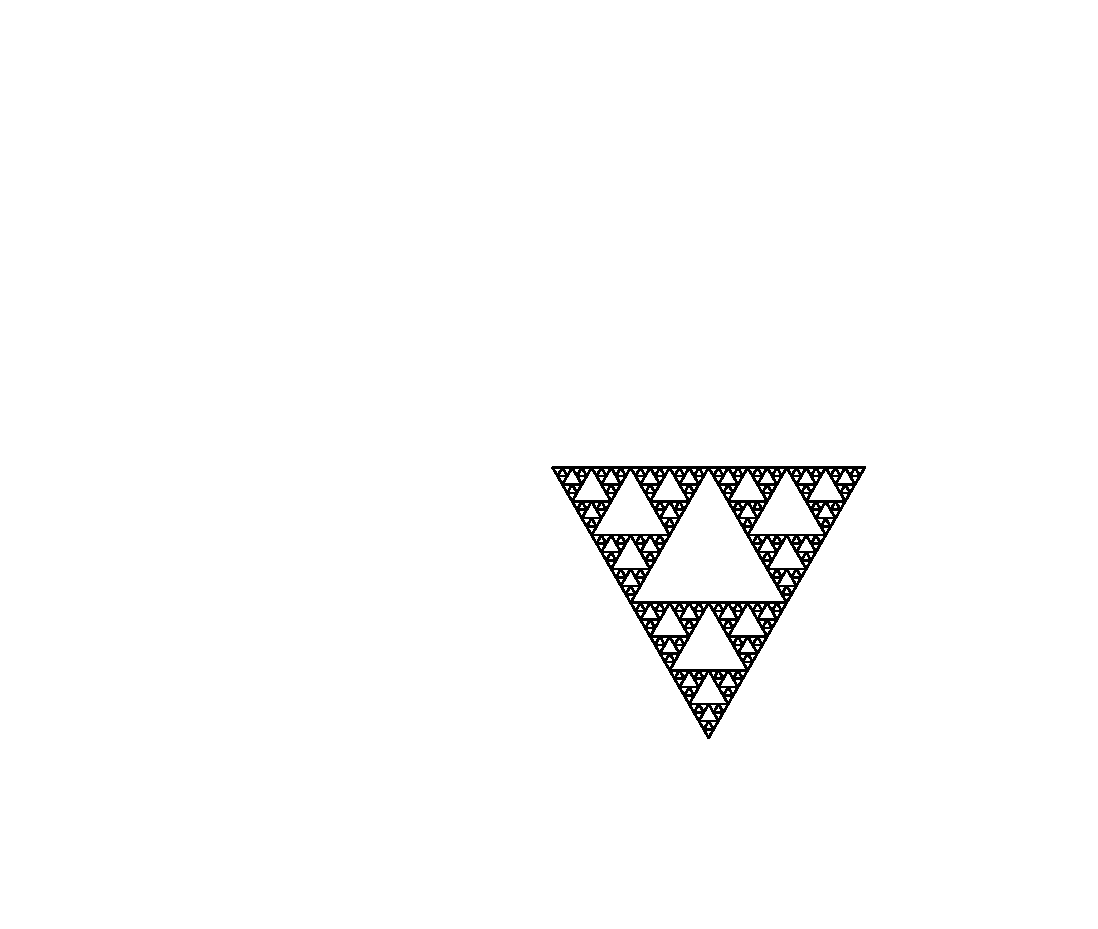
\includegraphics[width=0.6\textwidth]{triangle}
  \caption{Sierpinsky triangle with 5 subdivisions.}
\end{figure}
\subsection{Implementation and testing}
We used an iterative development process, meaning we started out by making a small piece of the code work in one iteration. Through testing, trial and error the goal of the iterative step was reached and we then carried on with the next step, where more code was implemented and tested. After several steps, we realized that our approach was overly complicated, so we started again from scratch. This time we did not care for optimization of the algorithm, and we solely focused on correctness.\footnote{The source code for this part of the porject can be found in the file \href{https://github.com/ErikAndersen81/DM550-FractalProject/blob/master/sierpinsky-triangle.py}{sierpinsky-triangle.py}}
\begin{figure}[H]
  \centering
  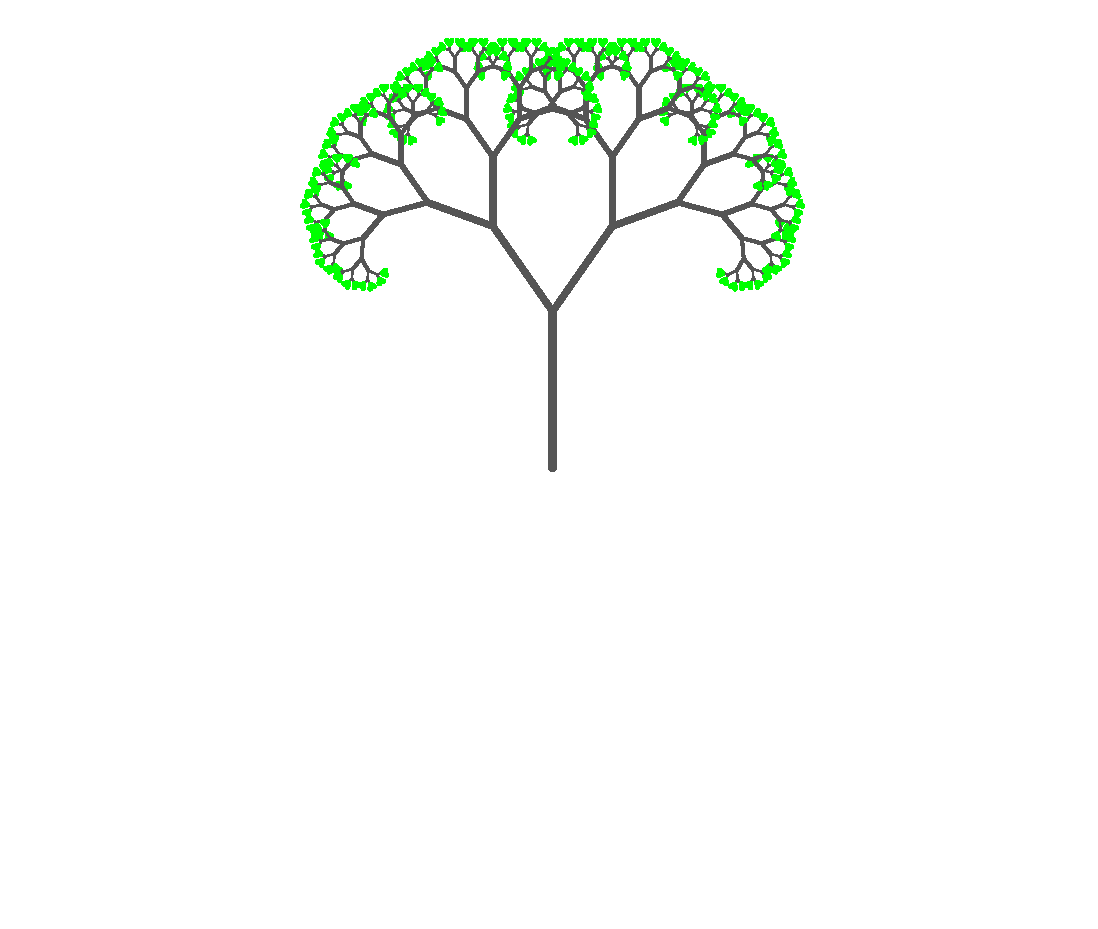
\includegraphics{bintree}
  \caption{Binary tree}
\end{figure}
\end{document}
